\documentclass{article}

\usepackage[utf8]{inputenc}
\usepackage[T2A]{fontenc}
\usepackage{amsmath}
\usepackage{fullpage}

\usepackage{tikz}
\usetikzlibrary{decorations}
\usetikzlibrary{decorations.pathmorphing}
\usetikzlibrary{decorations.pathreplacing}
\usetikzlibrary{decorations.shapes}

\begin{document}
    \renewcommand{\O}{\mathcal{O}}
    \newcommand{\floor}[1]{\left \lfloor #1 \right \rfloor}
    \newcommand{\parens}[1]{\left( #1 \right)}
    \newcommand{\brackets}[1]{\left[ #1 \right]}
    \newcommand{\braces}[1]{\left\{ #1 \right\}}

    \section{Задачи RMQ и LCA}
Динамическая задача RMQ/RSQ:
дерево отрезков, оценка $\O(log n)$
для запросов суммы/минимума
и изменения элемента.
Дерево отрезков.
Статический вариант задачи RMQ:
полное предвычисление
($\O(n^2)$ на предобработку, $\O(1)$ на запрос),
метод разреженной таблицы
($\O(n \log n)$ на предобработку, $\O(1)$ на запрос).
Задача LCA: эйлеров обход дерева,
сведение к задаче RMQ, двоичные подъёмы.
Сведение RMQ к ±1-RMQ.

    \section{Деревья поиска}
Корневое дерево:
бинарное дерево,
дерево с произвольным ветвлением,
представление <<левый ребёнок --- правый сосед>>.
Дерево поиска: поиск, вставка, удаление,
поиск следующего и предыдущего элемента за время,
пропорциональное высоте.
АВЛ-дерево: верхняя оценка $\O(\log n)$ на высоту,
сохранение свойства при помощи малых и больших вращений.

    \section{Splay-дерево}
Splay-дерево: дерево, которое остаётся сбалансированным
в среднем и при этом не хранит никакой
дополнительной информации в вершинах;
реализация основных операций через операцию splay;
верхняя оценка $\O(\log n)$ на среднюю стоимость операций.

    \section{Декартово дерево}
Декартово дерево: построение декартова дерева за линейное время
(при предварительно отсортированных ключах),
реализация операций вставки и удаления через split и merge.
Treap: верхняя оценка $\O(\log n)$ на мат. ожидание
глубины конкретной вершины, глубины средней вершины,
глубины дерева.
Использование неявного ключа, rope.

    \section{Хеширование}
Прямая адресация.
Коллизии.
Разрешение коллизий методом цепочек,
методом последовательных проб и методом двойного хеширования.
Гипотеза равномерного хеширования.
Оценка времени поиска в хеш-таблице при
использовании метода цепочек для гипотезы
равномерного хеширования.
Примеры хеш-функций.

    \section{Универсальные семейства хеш-функций}
Построение универсального семейства для
целочисленных ключей и для строк.
Оценка времени поиска в хеш-таблице
при использовании метода цепочек для универсального семейства.
Совершенное хеширование с помощью
универсального семейства хеш-функций.

\subsection{Конспект}
Множество функций $\cH$
из множества ключей $\mathcal{K}$
в $\{0, \ldots, m - 1\}$
называется
\emph{универсальным семейством хеш-функций},
если для любой пары различных ключей
$k_1$ и $k_2$
\[ \Pr_{h \in \cH} \brackets{h(k_1) = h(k_2)} \le \frac{1}{m} \]
(хеш-функция случайно выбирается один раз)

\begin{theorem}
    Среднее время безуспешного поиска в хеш-таблице при
    универсальном хешировании составляет $\Theta(1 + \alpha)$.
\end{theorem}
\begin{proof}
    \[
        X(i) =
        \begin{cases}
            1 & h(k_i) = h(k) \\
            0 & h(k_i) \ne h(k) \\
        \end{cases}
    \]

    По определению универсального семейства,
    и поскольку $k$ отсутствует в хеш-таблице
    $\E_h(X(i)) \le 1 / m$.

    Поэтому
    \begin{gather*}
        \E \brackets{\sum_{i=1}^n X(i)}
        = \sum_{i=1}^n \E X(i)
        \le \frac{n}{m} = \alpha
    \end{gather*}

    Хотя бы одно действие мы точно произведём,
    поэтому $\Theta(1 + \alpha)$.
\end{proof}

\begin{theorem}
    Среднее время успешного поиска в хеш-таблице при
    универсальном хешировании составляет $\Theta(1 + \alpha)$.
\end{theorem}
\begin{proof}
    Аналогично безуспешному поиску,
    но однин из $X(i)$ будет строго 1,
    поэтому
    \begin{gather*}
        \E \brackets{\sum_{i=1}^n X(i)}
        = \sum_{i=1}^n \E X(i)
        \le 1 + \frac{n - 1}{m} \in \Theta(1 + \alpha)
    \end{gather*}
\end{proof}

\subsection{Пример}
\begin{theorem}
    Путь $K = \{0, \ldots, n\}$.
    Выберем простое $p > n$.
    Тогда семейство $\cH$,
    состоящее из функций
    \[ h_{a, b}(k) = \Bigl( (ak + b) \Mod p \Bigr) \Mod m \]
    для $a = 1, \ldots, p - 1$ и $b = 0, \ldots, p - 1$
    будет универсальным.
\end{theorem}
\begin{proof}
    Рассмотрим $k_1 \ne k_2$.
    \begin{align*}
        & t_1 = (ak_1 + b) \Mod p &
        & t_2 = (ak_2 + b) \Mod p \\
    \end{align*}

    Т.к. $k_1 \ne k_2$, то $t_1 \ne t_2$.
    Если предположить, что $t_1 = t_2$,
    то
    \begin{gather*}
        ak_1 + b \equiv ak_2 + b \pmod{p} \\
        a(k_1 - k_2) \equiv 0 \pmod{p} \\
        a \ne 0 \Rightarrow k_1 = k_2
    \end{gather*}

    По $t_1, t_2, k_1, k_2$ можно однозначно восстановить $a, b$:
    \begin{gather*}
        t_1 - t_2 \equiv a(k_1 - k_2) \pmod{p} \\
        a \equiv (t_1 - t_2) \cdot (k_1 - k_2)^{-1} \pmod{p} \\
        b \equiv t_1 - a k_1 \pmod{p}
    \end{gather*}
    (кольцо по модулю $p$ --- поле, в нём есть деление).

    При всех возможных парах $a, b$
    каждая пара $t_1, t_2$ встречается ровно один раз.
    Тогда если выбирать $h_{a, b}$ случайно и равномерно из $\cH$,
    то пары $t_1, t_2$ будут случайно и равномерно
    распределены на $\{0, \ldots, p - 1\}$,
    при этом $t_1 \ne t_2$.

    Тогда вероятность того, что хеш-коды ключей совпадут,
    равна вероятности того, что два различных числа
    из $\{0, \ldots, p - 1\}$ окажутся равны по модулю $m$.
    Для фиксированного $t_1$ количество таких $t_2$ не превосходит
    \[
        \ceil{\frac{p}{m}} - 1
        \le \frac{p + m - 1}{m} - 1
        = \frac{p - 1}{m}
    \]

    Тогда вероятность получить коллизию равна
    \[
        \frac{1}{p} \cdot \frac{p - 1}{m} \le \frac{1}{m}
    \]
\end{proof}

\subsection{Совершенное хеширование}
Хотим для статического поиска иметь
поиск за строгое $\O(1)$
и $\O(n)$ памяти.
Для этого будем использовать таблицы второго уровня
с разными хеш-функциями вместо списков.
Скажем, что $n_i$ --- число ключей,
попавших в $i$-ю первичную ячейку.

\begin{theorem}
    \label{thm:06-1}
    При использовании универсального хеширования
    для хеш-таблицы размера $m = n^2$ вероятность
    возникновения коллизий не более $1/2$.
\end{theorem}
\begin{proof}
    Мат. ожидание количества коллизий
    \[
        \E X \le \binom{n}{2} \cdot \frac{1}{m}
        = \frac{n(n - 1)}{2} \cdot \frac{1}{n^2} < \frac{1}{2}
    \]

    По неравенству Маркова
    \[
        \Pr \brackets{X \geq 1} \le \frac{\E X}{1}
        < \frac{1}{2}
    \]
\end{proof}

\begin{theorem}
    \label{thm:06-2}
    При $m = n$
    \[
        \Pr \brackets{\sum_{i=0}^{n-1} n_i^2 \geq 4n} \le \frac{1}{2}
    \]
\end{theorem}
\begin{proof}
    Покажем, что
    \[
        \E \brackets{\sum_{i=0}^{n-1} n_i^2} < 2n
    \]

    \begin{gather*}
        n_i^2 = n_i + 2 \binom{n_i}{2} \\
        \E \brackets{\sum_{i=0}^{n-1} n_i^2}
        = \E \brackets{\sum_{i=0}^{n-1} n_i + 2 \sum_{i=0}^{n-1} \binom{n_i}{2}}
        = n + 2 \E \brackets{\sum_{i=0}^{n-1} \binom{n_i}{2}} \le \\
        \brackets{\text{вероятность коллизии не превосходит $1/m = 1/n$}} \\
        \le n + 2 \binom{n}{2} \cdot \frac{1}{n}
        = n + 2 \cdot \frac{n (n - 1)}{2} \cdot \frac{1}{n}
        = n + n - 1 < 2n
    \end{gather*}

    \[
        \Pr \brackets{\sum_{i=0}^{n-1} n_i^2 \geq 4n}
        \le \frac{\E \brackets{\sum_{i=0}^{n-1} n_i^2}}{4n}
        < \frac{2n}{4n} = \frac{1}{2}
    \]
\end{proof}

Тогда вероятностный алгоритм
построения совершенной хеш-таблицы:
\begin{enumerate}
    \item Построим хеш-таблицу $H$ и выберем хеш-функцию
    $h : K \to \{0, \ldots, m - 1\}$
    так, чтобы $\sum_{i=0}^{n-1} n_i^2 < 4n$.
    Для этого по теореме~\ref{thm:06-2} в среднем потребуется
    проверить не более двух хеш-функций.

    \item Когда такая $h$ найдена, для каждой $i$-й ячейки $H$
    заводим хеш-таблицу $T_i$ размера $n_i^2$
    и выбираем для неё хеш-функцию $g_i : K \to \{0, \ldots, n^2 - 1\}$
    так, чтобы у неё не было коллизий на множестве ключей,
    для которых $h(k) = i$.
    Для этого по теореме~\ref{thm:06-1} в среднем потребуется
    проверить не более двух хеш-функций.
\end{enumerate}

Полученный алгоритм построения работает за $\O(n)$,
требует $\O(n)$ памяти и даёт поиск за строгие $\O(1)$.

    \section{Числовые алгоритмы}
Cложение, умножение, деление длинных чисел.
Модульная арифметика: сложение, умножение,
возведение в степень, алгоритм Евклида,
расширенный алгоритм Евклида, деление.

\subsection{Алгоритмы арифметики}
Числа представляются как двоичные строки.
$n$ --- длина числа в битах.

Сложение --- очевидный алгоритм за $\O(n)$.

В процессорах умножение обычно
реализуется следующим алгоритмом в столбик
за $\O(n^2)$:
\begin{minted}{rust}
fn mul(mut a: Int, mut b: Int) -> Int {
    let mut r: Int = 0;
    for _ in 0..Int::BITS {
        if b & 1 == 1 {
            r += a;
        }
        a <<= 1;
        b >>= 1;
    }
    r
}
\end{minted}

Деление и получение остатка реализуется
алгоритмом в столбик
за $\O(n^2)$
(точнее, за $\O(n \cdot (n - m))$,
где $m$ --- старший бит $b$, считая с 0, $m < n$):
\begin{minted}{rust}
fn div_rem(mut a: Int, mut b: Int) -> (Int, Int) {
    let mut r: Int = 0;
    let mut maxbit = 0;
    for i in 0..Int::BITS {
        if b & (1 << i) != 0 {
            maxbit = i;
        }
    }
    for i in (0..Int::BITS - maxbit).rev() {
        let b = b << i;
        if a >= b {
            r |= 1 << i;
            a -= b;
        }
    }
    (r, a)
}
\end{minted}

Есть алгоритм Карацубы для умножения
за $\O(n^{\log_2 3})$.
Он основан на следующем:
\begin{gather*}
    (ax + b) \cdot (cx + d)
    = ac x^2 + (ad + bc) \cdot x + bd \\
    (a + b) \cdot (c + d)
    = ac + ad + bc + bd \\
    ad + bc = (a + b) \cdot (c + d) - ac - bd
\end{gather*}

Поэтому при дроблении задачи в 2 раза
достаточно провести 3 умножения частей
и $\O(1)$ сложений, а не 4 умножения,
т.е.
\begin{gather*}
    T(n) = 3 \cdot T(n/2) + \O(n) \\
    T(n) \in \O(n^{\log_2 3})
\end{gather*}

Существует алгоритм умножения,
основанный на быстром преобразовании Фурье,
за $\O(n \log n)$.

Базовый алгоритм Евклида:
\begin{minted}{rust}
fn gcd(a: Int, b: Int) -> Int {
    if a < b {
        gcd(b, a)
    } else if b == 0 {
        a
    } else {
        gcd(b, a - b)
    }
}
\end{minted}

Обычно пишут как
\begin{minted}{rust}
fn gcd(a: Int, b: Int) -> Int {
    if b == 0 {
        a
    } else {
        gcd(b, a % b)
    }
}
\end{minted}

\begin{theorem}
    Алгоритм Евклида находит НОД.
\end{theorem}
\begin{proof}
    Пусть $a = bq + r$.
    Пусть $a \equiv 0 \pmod c$
    и $b \equiv 0 \pmod c$.
    Тогда $r \equiv 0 \pmod c$,
    т.к. $r = a - bq$.
    Тогда множества общих делителей
    у $(a, b)$ и у $(b, r)$ совпадают.
\end{proof}

\begin{theorem}[Теорема Безу]
    Всегда существуют целые $x$ и $y$
    такие, что $ax + by = \gcd(a, b)$.
\end{theorem}
\begin{proof}
    Расширенный алгоритм Евклида.
    \begin{minted}{rust}
    fn gcd_ext(a: Int, b: Int) -> (Int, Int, Int) {
        if a < b {
            let (g, x, y) = gcd_ext(b, a);
            (g, y, x)
        } else if b == 0 {
            (a, 1, 0)
        } else {
            let (g, x, y) = gcd_ext(b, a - b);
            (g, y, x - y)
        }
    }
    \end{minted}
\end{proof}

Расширенный алгоритм Евклида можно записать через модуль:
\begin{minted}{rust}
fn gcd_ext_mod(a: Int, b: Int) -> (Int, Int, Int) {
    if b == 0 {
        (a, 1, 0)
    } else {
        let q = a / b;
        let (g, x, y) = gcd_ext_mod(b, a % b);
        (g, y, x - q * y)
    }
}
\end{minted}

\begin{theorem}
    $|x| \le b$ и $|y| \le a$
\end{theorem}
\begin{proof}
    Если $a \equiv 0 \pmod b$,
    то рекурсивный вызов вернёт $(b, 1, 0)$.

    По индукции предположим, что для рекурсивного вызова выполняется.
    Тогда
    \begin{gather*}
        q = \floor{\frac{a}{b}} \\
        r = a \Mod b \\
        \gcd(a, b) = x' \cdot b + y' \cdot r \\
        |x'| \le r \\
        |y'| \le b \\
        x = y' \\
        y = x' - qy' \\
        |x| = |y'| \le b \\
        |y| \le |x'| + |qy'| \le r + qb = a
    \end{gather*}
\end{proof}

Возведение в степень --- алгоритм за $\O(M \log p)$,
где $M$ --- сложность умножения, а $p$ --- степень.

\subsection{Модульная арифметика}
Сложение, умножение, степень --- очевидно.

Деление --- через расширенный алгоритм Евклида
и поиск обратного:
\begin{gather*}
    a / b = a \cdot b^{-1} \\
    b \cdot b^{-1} \equiv 1 \pmod m \\
\end{gather*}

Для существования такого $q$ нужно,
чтобы $\gcd(b, m) = 1$, т.к. иначе
$1 \ne \gcd(b, m) \mid bq$.

Воспользуемся расширенным алгоритмом Евклида и найдём $x$ и $y$:
\[ bx + my \equiv bx \equiv 1 \pmod m \]
это $x$ и будет искомым $q$.
Нужно модифицировать $\gcd$ для использования модульного
сложения и умножения:
\begin{minted}{rust}
fn gcd_ext_mod(a: Int, b: Int, m: Int) -> (Int, Int, Int) {
    if a < b {
        let (g, x, y) = gcd_ext_mod(b, a, m);
        (g, y, x)
    } else if b == 0 {
        (a, 1, 0)
    } else {
        let (g, x, y) = gcd_ext_mod(b, (a + m - b) % m, m);
        (g, y, (x + m - y) % m)
    }
}
\end{minted}

Если $m$ --- простое, то обратный элемент есть всегда.

    \section{Простые числа}
Проверка чисел на простоту.
Числа Кармайкла, малая теорема Ферма.
Генерация случайных простых чисел.
Криптография: схемы с закрытым ключом, RSA.
Необходимые факты теории чисел.

    \section{Быстрое преобразование Фурье}
Быстрое вычисление значений многочлена в точках:
два способа задания многочленов
--- коэффициентами и значениями в точках;
вычисление значений многочлена в точках методом
<<разделяй и властвуй>>;
дискретное преобразование Фурье;
быстрое преобразование Фурье.
Интерполяция: интерполяция в терминах матриц;
матрица Вандермонда;
интерполяция как домножение на обратную матрицу.
Необходимые факты линейной алгебры.

\subsection{Конспект}
Многочлен степени $d$ однозначно задаётся $d + 1$ точкой,
доказательство --- метод интерполяции.
Произведение двух многочленов степени $d$ ---
многочлен степени $2d$.

Заметим, что если мы выбираем точки вида
$x_{2k} = -x_{2k - 1}$,
то можно разделить многочлен
$P(x) = a_0 + a_1 x + a_2 x^2 + \ldots$
в виде $P(x) = P_0(x) + x \cdot P_1(x)$,
где $P_0(x) = a_0 + a_2 x^2 + \ldots$,
а $P_1(x) = a_1 + a_3 x^2 + \ldots$.
Тогда можно посчитать $P(x)$ и $P(-x)$ вместе:
\begin{align*}
    P(x) & = P_0(x) + x \cdot P_1(x) \\
    P(-x) & = P_0(-x) - x \cdot P_1(-x) = \\
    & = P_0(x) - x \cdot P_1(x) \\
\end{align*}

Именно так работает быстрое преобразование Фурье,
только $x$ берутся нетривиальными корнями из 1.
Обычно --- в комплексных числах:
\begin{center}
    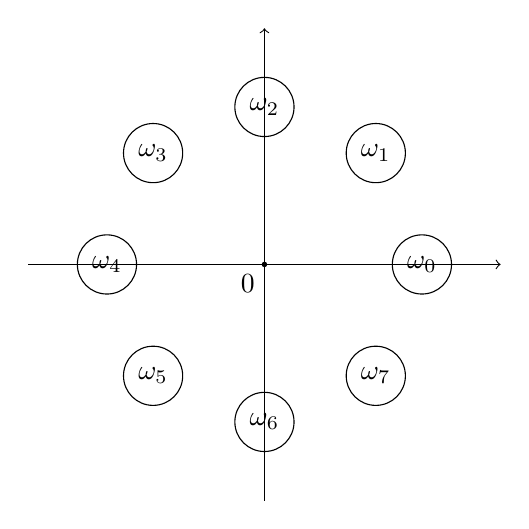
\begin{tikzpicture}
        \foreach \w in {0,...,7} {
            \node[draw,circle] (w\w) at (45*\w : 2cm) {$\omega_{\w}$};
        }
        \draw[->] (-3,0) -- (3,0);
        \draw[->] (0,-3) -- (0,3);
        \fill (0,0) circle (1pt);
        \node[anchor=north east] at (0,0) {$0$};
    \end{tikzpicture}
\end{center}

То есть для $j = 2k \Mod n$
выполняется $\omega_j = \omega_k^2$
и $n = 2^q$.
Иными словами,
$\omega_i = \exp \parens{\frac{2 \pi i}{n}}$.

FFT позволит быстро посчитать точки:

\noindent
\begin{minipage}{\textwidth}
    \begin{algorithmic}
        \State $\omega_N(i) = \exp \parens{\frac{2 \pi i}{N}}$
        \Function{fft}{$n=N, k=0, \Delta=1$}
            \Comment{$k$ --- индекс, $\Delta$ --- шаг индекса}
            \If{$n = 1$}
                \Return $P[k]$
            \EndIf
            \State $P_0(\omega^{2j}) = \Call{fft}{n / 2, k, 2 \Delta}$
            \State $P_1(\omega^{2j}) = \Call{fft}{n / 2, (k + \Delta) \Mod N, 2 \Delta}$
            \For{$j = 0, \ldots, n - 1$}
                \State $P(\omega^j) = P_0(\omega^{2j}) + \omega^j \cdot A_1(\omega^{2j})$
            \EndFor
            \Return $P(\omega^j)$
        \EndFunction
    \end{algorithmic}
\end{minipage}

Очевидно, \textsc{fft} работает за $\O(N \log N)$.

Матричный вид, т.н. матрица Вандермонда:

\[
    \begin{bmatrix}
        P(x_0) \\
        P(x_1) \\
        \ldots \\
        P(x_{n - 1}) \\
    \end{bmatrix}
    =
    \begin{bmatrix}
        1 & x_0 & x_0^2 & \ldots & x_0^{n - 1} \\
        1 & x_1 & x_1^2 & \ldots & x_1^{n - 1} \\
        & & \vdots & & \\
        1 & x_{n - 1} & x_{n - 1}^2 & \ldots & x_{n - 1}^{n - 1} \\
    \end{bmatrix}
    \cdot
    \begin{bmatrix}
        a_0 \\
        a_1 \\
        \ldots \\
        a_{n - 1} \\
    \end{bmatrix}
\]

Интерполяцию можно реализовать домножением на обратную матрицу:
\[
    \frac{1}{n}
    \cdot
    \begin{bmatrix}
        1 & 1 & \ldots & 1 \\
        \omega_0^{-1} & \omega_1^{-1} & \ldots & \omega_{n - 1}^{-1} \\
        \omega_0^{-2} & \omega_1^{-2} & \ldots & \omega_{n - 1}^{-2} \\
        & & \vdots & & \\
        \omega_0^{1 - n} & \omega_1^{1 - n} & \ldots & \omega_{n - 1}^{1 - n} \\
    \end{bmatrix}
    \cdot
    \begin{bmatrix}
        1 & \omega_0 & \omega_0^2 & \ldots & \omega_0^{n - 1} \\
        1 & \omega_1 & \omega_1^2 & \ldots & \omega_1^{n - 1} \\
        & & \vdots & & \\
        1 & \omega_{n - 1} & \omega_{n - 1}^2 & \ldots & \omega_{n - 1}^{n - 1} \\
    \end{bmatrix}
    = ?
\]

Рассмотрим отдельную ячейку $i, j (i \ne j)$:
\[
    \frac{1}{n}
    \sum_{k=0}^{n - 1}
    \omega_k^{-i}
    \cdot
    \omega_k^j
    =
    \frac{1}{n}
    \sum_{k=0}^{n - 1}
    \omega_1^{k(j - i)}
    =
    \frac{1}{n}
    \cdot
    \frac{1 - \omega_1^{n(j - i)}}{1 - \omega_1^{j - i}}
    =
    0
\]

\[
    \frac{1}{n}
    \sum_{k=0}^{n - 1}
    \omega_k^{-j}
    \cdot
    \omega_k^j
    =
    1
\]

Т.е. на главной диагонали единицы,
в остальных ячейках нули.
Получили обратную матрицу.

    \section{Задача линейного программирования и симплекс-метод}
Линейное программирование.
Общий вид задачи, матричная форма и
сведение между различными представлениями.
Вершины: равносильность двух определений и достижение максимума.
Симплекс-метод, нахождение начальной точки.
Двойственность: построение двойственной
задачи, теорема о двойственности --- слабая (с доказательством)
и сильная (без доказательства) формулировки.

\subsection{Задача}
Есть набор переменных, нужно присвоить им вещественные значения
с учётом линейных ограничений
и максимизируя / минимизируя линейную функцию.

\begin{align*}
    &
    \left\{
    \begin{aligned}
        & \sum_{i=1}^n c_i x_i = \max \\
        & \forall j \in \{1, \ldots, m\}.~\sum_{i=1}^n a_{ji} x_i \le b_j \\
        & \forall i \in \{1, \ldots, n\}.~x_i \ge 0 \\
    \end{aligned}
    \right.
    &&
    \left\{
    \begin{aligned}
        C^T \cdot X & = \max \\
        A \cdot X & \le B \\
        X & \ge 0 \\
    \end{aligned}
    \right.
\end{align*}

Пример --- максимизация прибыли,
если на складе есть материалы,
из которых производятся товары
заранее известной стоимости.

Стоит обратить внимание, что неравенства нестрогие.

\subsection{Разные виды}
\begin{itemize}
    \item Целевая функция максимизируется или минимизируется
    (эквивалентно, т.к. просто $c_i$ разного знака);

    \item Ограничения неравенством или равенством:
    для $\sum_{i=1}^n a_i x_i \le b$
    вводим $s$ и пишем
    \[
        \left\{
        \begin{aligned}
            & \sum_{i=1}^n a_i x_i + s = b \\
            & s \ge 0 \\
        \end{aligned}
        \right.
    \]

    Обратно --- для $A = B$ пишем $A \le B$ и $A \ge B$ ($-A \le -B$);

    \item Неограниченная переменная сводится к двум неотрицательным:
    $x = x^+ - x^-$, $x^+ \ge 0$, $x^- \ge 0$.
\end{itemize}

\paragraph{Стандартный вид:}
целевая функция минимизируется,
все переменные неотрицательные,
ограничения --- уравнения.

Линейные ограничения задают гиперплоскости,
которые содержат грани полиэдра (многогранника),
в котором лежат все точки, попадающие под ограничения.
Ограничения могут быть не замкнуты,
тогда функция может быть бесконечной,
либо точек, попадающих под ограничения,
может не быть.
Если же ограничения замкнуты,
тогда ответ лежит в одной из вершин.

Симплекс-метод:
найти некоторую вершину,
дальше идти в сторону тех соседей,
для которых целевая функция увеличивается.

    \section{Целочисленное линейное программирование}
ILP: пример для максимального паросочетания
и вершинного покрытия в двудольном графе.
Тотальная унимодулярность:
определение и почему это гарантирует целочисленность решения.
Доказательство теоремы Кёнига через двойственность.

\subsection{Двудольный граф}
Максимальное паросочетание:
каждому ребру $e_j$ назначим $x_j$
--- берём или нет это ребро,
и задача выглядит так:
\begin{eqnsystem}
    & \sum_{j=1}^{|E|} x_j \to \max \\
    & \forall i \le |V|.~\sum_{j=1}^{|E|} a_{ij} x_j \le 1 \\
    % & \forall j \le |E|.~x_j \le 1 \\
    & \forall j \le |E|.~x_j \ge 0 \\
\end{eqnsystem}
где $a_{ij}$ --- инцидентность вершины $v_i$ ребру $e_j$.

Минимальное вершинное покрытие:
каждой вершине $v_i$ назначим $y_i$
--- берём или нет эту вершину.
Задача выглядит так:
\begin{eqnsystem}
    & \sum_{i=1}^{|V|} y_i \to \min \\
    & \forall j \le |E|.~\sum_{i=1}^{|V|} a_{ij} y_i \ge 1 \\
    % & \forall i \le |V|.~y_i \le 1 \\
    & \forall i \le |V|.~y_i \ge 0 \\
\end{eqnsystem}
где $a_{ij}$ --- инцидентность вершины $v_i$ ребру $e_j$.

\begin{theorem}[теорема Кёнига]
    Максимальное паросочетание не больше минимального вершинного покрытия
\end{theorem}
\begin{proof}
    См. задачи линейного программирования выше,
    можно заметить, что если
    $A$ --- матрица инцидентности
    (т.е. $a_{ij}$ --- инцидентность $v_i$ и $e_j$),
    то задачи выглядят как
    \begin{align*}
        &
        \begin{system}
            & 1_{|E|}^T \cdot X \to \max \\
            & A \cdot X \le 1_{|V|} \\
            & X \ge 0 \\
        \end{system}
        &&
        \begin{system}
            & 1_{|V|}^T \cdot Y \to \min \\
            & A^T \cdot Y \ge 1_{|E|} \\
            & Y \ge 0 \\
        \end{system}
    \end{align*}
    Т.е. задачи двойственны друг другу,
    следовательно,
    оптимум минимального вершинного покрытия
    равен оптимуму максимального паросочетания.
\end{proof}

\subsection{Унимодулярность}
Тотальная унимодулярность:
определитель каждой квадратной подматрицы
(в т.ч. с пробелами) --- $\pm 1$ или $0$.
\begin{theorem}
    Все вершины многогранника с тотально унимодулярной
    матрицей целочисленны.
\end{theorem}
\begin{proof}
    Рассмотрим вершину $(x_1, \ldots, x_n)$.
    Её система уравнений:
    \begin{eqnsystem}
    \end{eqnsystem}
\end{proof}

    \section{Задача о максимальном потоке}
Задача о максимальном потоке.
Теорема о минимальном разрезе и максимальном потоке.
Алгоритм Форда-Фалкерсона.
Алгоритм Эдмондса-Карпа (без доказательства корректности).
Двудольное паросочетание через потоки.

    \section{Поиск подстроки в строке}
Наивный алгоритм.
Алгоритм Рабина-Карпа.
$z$-функция, префикс-функция,
алгоритм Кнута-Морриса-Пратта.

    \section{Структура бор}
Бор. Алгоритм Ахо-Корасик.

    \section{Суффиксные структуры}
Суффиксное дерево: определение, поиск подстроки.
Суффиксный массив: определение, поиск подстроки,
построение за $\O(n \log n)$.

    \section{NP-полные задачи}
Определение классов P и NP.
Полиномиальные сведения.
NP-полнота задачи выполнимости булевой схемы.
Сведение CircuitSAT к SAT.
Сведение SAT к 3SAT.
Сведение 3SAT к IndependentSet.
Сведение IndependentSet к VertexCover и Clique.
Неразрешимость Halting Problem.

\subsection{Конспект}
Задача поиска полиномиально сводится к задаче проверки существования.
Сначала проверяем существование без ограничений,
потом ограничиваем первый бит,
потом второй, и т.д.

Задачи P (polynomial) --- у которых существует
полиномиальный алгоритм решения.

Задачи NP (non-deterministic polynomial) --- у которых существует
полиномиальный алгоритм проверки решения
(и решение полиномиального размера от входа).
Проверяемое решение --- <<сертификат>> (подсказка).

Пример P: эйлеров цикл.
Пример NP: гамильтонов цикл.

NP-hard --- к задаче можно полиномиально свести любую из NP.
Например, проблема останова --- NP-hard.
NP-complete --- NP-hard, находящаяся в NP.

Неизвестно, возможно ли решить
SAT (Satisfiability) быстрее $\O*(2^n) = \O(2^n \cdot Poly(n))$.
Можно решить k-SAT за $\O(2^{\varepsilon_k n}) \mid \varepsilon_k < 1$.
Для k = 2 существует линейное решение.

SAT => 3-SAT: возьмём конъюнктивную нормальную форму
\[
    (x_1 \lor \ldots \lor x_n) \land \ldots
    \Leftrightarrow
    (x_1 \lor x_2 \lor y_1) \land
    (\lnot y_1 \lor x_3 \lor y_2) \land \ldots \land
    (\lnot y_{n - 2} \lor x_{n - 1} \lor x_n) \land \ldots
\]
Если хотя бы один $x_i$ положителен,
то от него распространяются $y_j$ влево и вправо.
Если нет, то нельзя найти $y_j$, чтобы выражение выполнялось.

3SAT в независимое множество:
сделаем группы вершин (не соединённых),
соответствующих всем конъюнктам.
Вершины --- литералы,
рёбра --- между литералами одного конъюнкта
и между $x$ и $\lnot x$.
Тогда решением 3SAT было бы независимое множество
такого же размера, как количество конъюнктов.

Vertex Cover: если нашли вершинное покрытие,
то оставшиеся вершины --- независимое множество,
и наоборот.
Поэтому вершинное покрытие --- инверсия независимого множества.

Clique: независимое множество в графе
--- это клика в дополнении этого графа,
и наоборот.

Проблема останова неразрешима:
пронумеруем все алгоритмы,
пусть алгоритм $A$ определяет,
завершится ли алгоритм $B$ на входе $C$.
Тогда найдём алгоритм $D$,
который берёт некоторый ввод $E$,
запускает алгоритм $A$ с $B = C = E$
и инвертирует результат.
Запустим $D(D)$.
Если $A$ говорит, что $D(D)$ должен завершиться,
то $D$ не завершится, а если наоборот, то должен.
Следовательно, парадокс.

    \section{Методы решения NP-полных задач}
Методы решения NP-полных задач.
Backtracking, Branch \& Bound, параметризованные алгоритмы.
Приближенные алгоритмы для NP-полных задач.
2-приближенный алгоритм для вершинного покрытия.
2-приближенный алгоритм для метрического коммивояжёра.
Алгоритм Кристофидеса-Сердюкова.
Константное приближение TSP влечёт P = NP.
$\log(n)$-приближенный алгоритм для покрытия множествами.
Формулировка жадной гипотезы о надстроке.

\subsection{Конспект}
TSP --- задача коммивояжёра:
существует ли простой цикл,
проходящий через все вершины.

\bigskip

2-приближённый вершинного покрытия
--- смотрим на каждое ребро, если оно уже покрывается,
то всё ок, если нет, то берём обе его вершины.

\bigskip

Метрическая TSP: на входе полный граф,
веса между вершинами --- расстояния (математические).
Тогда 2-приближением будет построить MST,
провести обход по нему в порядке DFS,
и удалить повторения вершин из пути.
Истинный кратчайший путь $S$
как минимум содержит в себе какое-то
остовное дерево, следовательно,
не меньше MST.
А путь, который мы нашли, это удвоенное MST.

\bigskip

Алгоритм Кристофидеса-Сердюкова:
в $T$ количество вершин нечётной степени чётно.
Найдём совершенное паросочетание
минимального веса (не умеем это делать) $M$
на этих вершинах
и добавим его рёбра в $T$,
получился мультиграф с вершинами чётной степени.
Теперь существует эйлеров цикл,
возьмём его и удалим повторы.

$2 |M| \le |S|$:
построим два паросочетания $M_1$ и $M_2$ на вершинах $M$,
идя по $S$ и чередуя рёбра (т.е. $M_1 \cup M_2 \subset S$).
Тогда $|M_1| + |M_2| \le |S|$,
а $|M| \le \min(|M_1|, |M_2|)$.
Следовательно, это будет $3/2$-приближением.

\begin{theorem}
    Если существует константное приближение
    произвольной задачи коммивояжёра
    (т.е. не обязательно метрическое)
    с путём вместо цикла,
    то P = NP.
\end{theorem}
\begin{proof}
    Сведём поиск гамильтонова пути к задаче коммивояжёра.
    Из заданного графа $G$ построим полный граф $H$
    следующим образом:
    \[
        w(u \to v) =
        \begin{cases}
            1 & u \to v \in E \\
            \alpha \cdot n & u \to v \notin E \\
        \end{cases}
    \]

    Пусть $\mathcal{A}(H)$ --- $\alpha$-приближение $TSP(H)$.

    Тогда если гамильтонов путь существует, то
    \begin{align*}
        TSP(H) & = n - 1 \\
        \mathcal{A}(H) & \le \alpha \cdot (n - 1) \\
    \end{align*}

    В противном случае
    \begin{align*}
        TSP(H) & \ge \alpha n \\
        \mathcal{A}(H) & \ge \alpha n > \alpha \cdot (n - 1) \\
    \end{align*}

    Таким образом, существование $\alpha > 0$-сведения
    задачи коммивояжёра о пути на полном графе
    позволяет за полином решить NP-полную задачу
    о гамильтоновом пути.
\end{proof}

(более очевидно, если будем доказывать через гамильтонов цикл)

\subsection{Покрытие множествами}
Есть множество $U$ элементов,
нужно найти такой минимальный набор из заданных подмножеств $S_i$,
что всё множество будет покрыто.

Жадно берём наибольшее множество $S_j$ из заданных подмножеств,
затем из всех имеющихся множеств удаляем покрытые им элементы:
\begin{algorithmic}
    \State $U \gets U \setminus S_j$
    \State $S_i \gets S_i \setminus S_j$
\end{algorithmic}

\begin{theorem}
    Если истиный размер покрытия --- $k$,
    то размер найденного покрытия не больше $k \ln n$.
\end{theorem}
\begin{proof}
    Пусть $U_t$ --- оставшиеся непокрытыми элементы после $t$-го шага,
    $|U_t| = n_t, U_0 = U$.
    Тогда на каждой итерации существует покрытие
    $U_t$ $k$ оставшимися множествами, следовательно,
    $\exists i.~|S_i \cap U_t| \ge n_t / k$.
    Тогда
    \[
        n_t
        \le n_{t - 1} \cdot \parens{1 - \frac{1}{k}}
        \le \ldots
        \le n \cdot \parens{1 - \frac{1}{k}}^t
        = n \cdot \parens{1 - \frac{1}{k}}^{k \cdot \frac{t}{k}}
        < n \cdot \exp \parens{-\frac{t}{k}}
    \]

    Как только $n_t < 1$, получили покрытие.
    \begin{align*}
        n_t & < n \cdot \exp \parens{-\frac{t}{k}} < 1 \\
        & \Rightarrow n < \exp \parens{\frac{t}{k}} \\
        & \Rightarrow \ln n < \frac{t}{k} \\
        & \Rightarrow t > k \ln n
    \end{align*}
    То есть если сделали $\ceil{k \ln n}$ шагов,
    то все элементы покрыты.
    Размер ответа --- $\ceil{k \ln n}$.
\end{proof}

\subsection{Жадная гипотеза о надстройке}
Есть словарь $S_i$, нужно найти минимальную строку $S$,
что все строки из словаря --- её подстроки.
Гипотеза: жадный алгоритм даёт 2-приближение.

Жадный алгоритм: на каждом шаге берём две строки
с максимальным наложением и заменяем их на их склейку в словаре.

Лучший известный алгоритм с доказанной оценкой
даёт $2\frac{11}{23}$-приближение.

    \section{Альтернативные модели вычисления}
Модель внешней памяти.
Сортировка слиянием в модели внешней памяти.
Модель cache-oblivious.
Модель PRAM, вычисление максимума за константу.
Модель BSP.
Сортировка методом регулярного сэмплирования.

\end{document}
